\section{基于知识增强的常识性推理研究}
在本研究中,我们致力于解决常识推理领域的关键挑战:增强模型的常识性推理能力。
在\secref{sec1:related}中,我们已经深入探讨了当前领域内的领先技术,特别是BERT等先进
的神经网络方法。尽管神经网络在常识推理任务中已显示出卓越的性能,
但根据Lin等人的研究\cite{lin2020birds,peng2022copen},在精确处理和表达常识性知识方面,
这些方法仍有进一步提升的空间。

针对这一挑战,我们选择了一个具有挑战性的任务作为研究重点:预测叙事故事的结局。这一
任务的灵感源自早期的故事理解研究\cite{meehan1977tale},并随时间演进,扩展为预测故
事中可能事件的任务\cite{chambers2008unsupervised}。我们的实验是在ROC故事填
空测试数据集\cite{mostafazadeh2016corpus}上进行的,这一数据集为我们提供了评
估模型性能的有效平台。

为了在这一领域实现突破,我们提出了一种注重故事中关键概念识别与
优化的新方法。这种方法通过专注于故事的关键元素,而非全体词汇,旨在简化句
子结构,减少干扰信息,从而提升模型在捕捉故事核心内容方面的效能。此外,我们
采用了一种将结构化的常识知识融入句子表达的策略,通过结合结构化预训
练的概念嵌入(embedding),增强
了模型在理解故事情境与结局之间关键概念联系的能力。

通过将这些精细化的概念与丰富结构化知识相结合,我们不仅深化了对故事情节的理解,
也在故事推理任务的准确度上取得了显著的提升。这一成果标志着我们在常识推理任务
处理方面迈出了重要的一步。

\subsection{概述}
\label{sec2:intro}
在叙事故事中预测``接下来会发生什么''是人工智能中常识推理的一个重要并且富有挑战性的任务。
故事理解最初在规划和目标搜索的背景下被研究~\cite{meehan1977tale},这是人工智能中最重要的问题之一。
随着研究的深入,这一任务逐渐演变为预测故事中可能接踵
而至的事件~\cite{chambers2008unsupervised}。众多研究聚焦于一个标准数据集
——故事填空测试(ROC)~\cite{mostafazadeh2016corpus}。这个挑战要求从两个备选
结局中选出一个与四句话故事情境最为吻合的结局,如\figref{fig:story}(a)所示。

\begin{figure}[th]
  \centering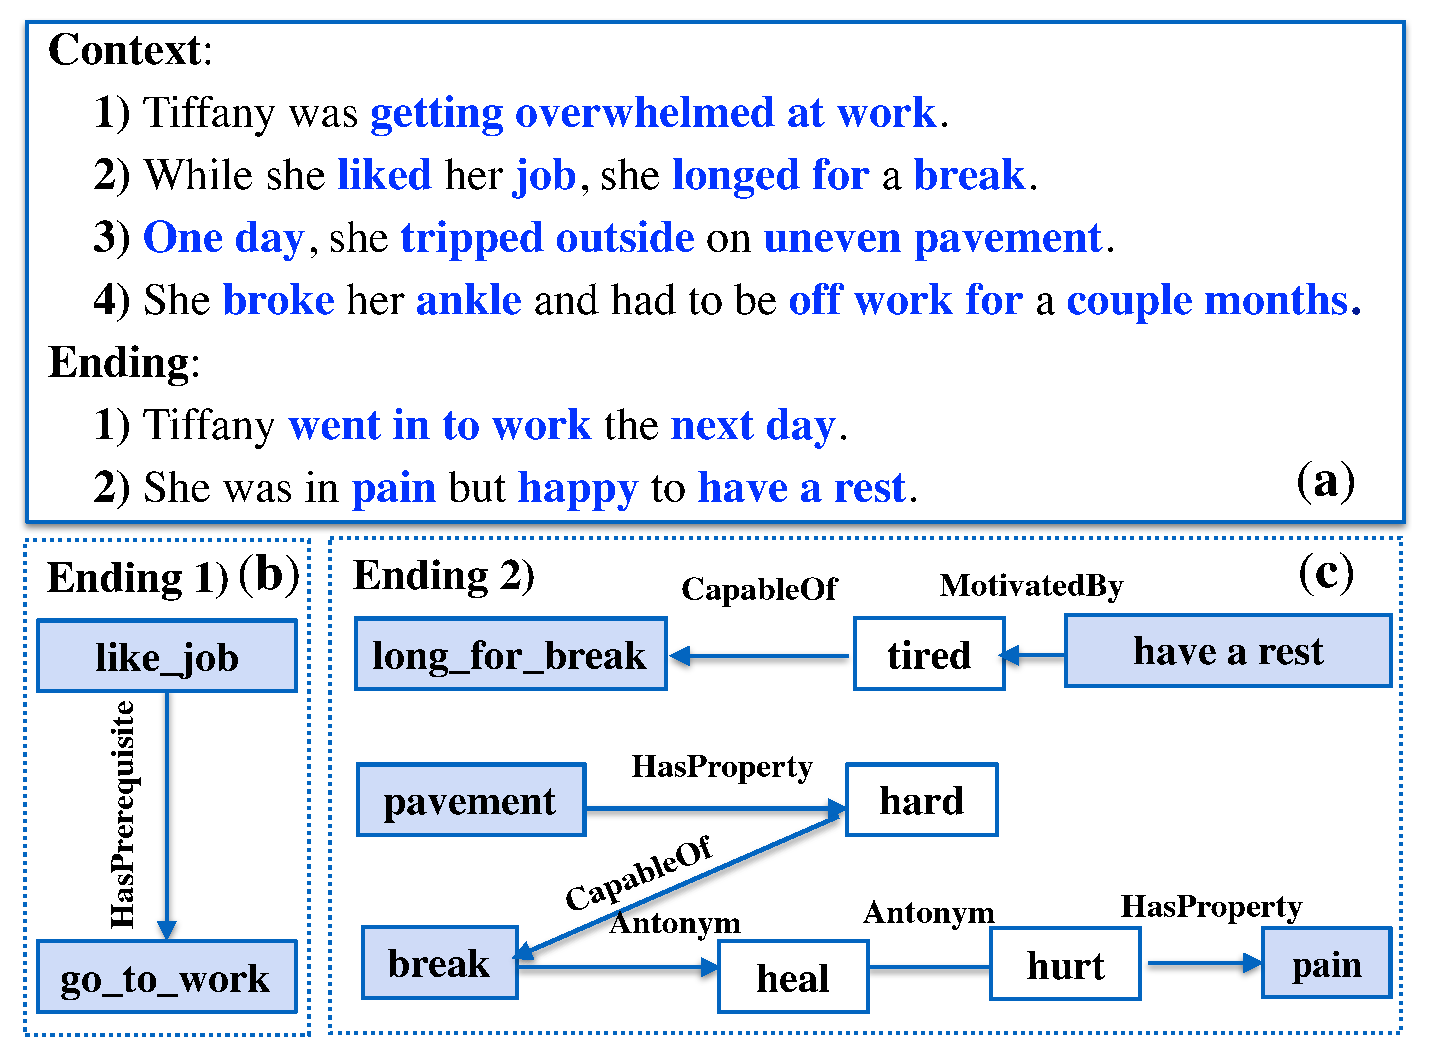
\includegraphics[width=4in]{figures/story/story_example}
  \caption{故事填空任务中的一个例子。在(b)和(c)中,蓝色框内的单词代表故事中的关键概念;白色框内的单词虽非故事概念,但作为桥接节点发挥作用。}
  \label{fig:story}
  \end{figure}

先前的研究成果表明,结构化的常识知识对于深化故事理解颇具
帮助~\cite{li2019story}。例如,观察\figref{fig:story}(b)和(c),我们
不难发现,结构化知识有助于通过分析词汇间的逻辑联系来推断故事的
可能结局。更有趣的是,仅凭
借关键词(在图中以蓝色高亮显示)就能做出推理,这些词汇在推理过程中提
供了丰富信息,而无需解析全文。相对而言,其他未突出显示的词汇不仅信息量较少,
甚至可能由于其模糊的语义而对分类器造成干扰。例如,``Tiffany''这一名字常与珠宝相关联,
将这层含义引入故事情境中,往往会产生负面效果。

受以上观察的启发,我们从两个方面运用常识知识来优化故事的表达方式。
首先,我们通过从ConceptNet~\cite{speer2017conceptnet}中提炼关键概念,对
句子进行简化处理。ConceptNet作为一个社区策划的开放领域知识图谱,涵盖了绝大多数
常识推理所需的知识,从而实现了{\em 句内}概念的有效表示。其次,我们通过
融入ConceptNet知识图谱中的预训练概念嵌入,将结构化的常识知识引入故事句
子的表达中。例如,在\figref{fig:story}(c)中,``long for break''与``have a rest''之间
通过{\em CapableOf}和{\em MotivatedBy}关系边相连。这些连接为我们在故事中``串联起关键点'',帮
助我们进行更加深入和有意义的推理分析。

%在面对常识推理任务中的首个挑战(\ref{sec1:challenge}节):提升模型常识性推理能力的挑战时,
%本研究聚焦于当前最为前沿的方法——神经网络方法(\ref{sec1:approachs}节),
%并对其进行了深入分析。尽管神经网络在常识推理任务中表现出色,
%但有工作\cite{lin2020birds}指出,在处理常识性知识时,这些方法仍有改进空间,
%特别是在准确把握和表达常识性知识方面。为了在这一领域取得进一步突破,
%我们选择了一个具有挑战性的任务——``预测叙事故事结尾''。
%这一任务源自早期关于故事理解的研究\cite{meehan1977tale},
%后演变为预测故事中可能发生事件的任务\cite{chambers2008unsupervised}。
%本研究在 ROC 数据集\cite{mostafazadeh2016corpus},也就是故事填空数据集,
%上进行了实验评估,该数据集要求从两个备选结局中选择一个与四句话故事情境最为契合的结局。

%最初的故事填空测试尝试主要集中在计算候选结局与故事情境句子间的语义相似度上。
%这通常需要对故事句子进行某种形式的表示,如通过平均句子中的词
%向量\cite{mikolov2013distributed},应用sentence2vec\cite{kiros2015skip},
%DSSM\cite{huang2013learning}或其他特征\cite{schwartz2017story}。近期的方法
%更倾向于采用两层架构:首先使用LSTM\cite{hochreiter1997long},GPT\cite{radford2018improving}或BERT\cite{devlin2018bert}等预训练语言
%模型从庞大的语料库中构建每个句子的表示,然后在ROC数据集上对分类模型进行微调,
%以融合成完整的故事情境表示。



%在这些方法中,故事的完整句子被采用。早期模型对
%句子中的每个单词平等对待,而后续更先进的语言模型,如基于
%注意力机制的模型,为不同单词赋予了不同的权重。这些权重通常是从
%大型语料库中隐式学习得到的,而常识性知识在其中虽然存在,但相对稀
%疏。从\figref{fig:story}(a)中可以看出,通过专注于关键词(用蓝色高亮表示)而
%非所有单词,可以更准确地找到正确的结局。实际上,其他未高亮的单词可能因其
%模糊不清的含义而干扰下游分类器。例如,提及``Tiffany''这个名字可能会误导读者
%联想到珠宝,从而对故事情境产生不利影响。

%基于这些观察,我们提出在使用语言模型表示之前,通过保留被认为重
%要的标记来简化句子,即将不重要的标记的权重降至零。我们将句子建模为一系列
%事件和概念,这些概念在ConceptNet\cite{speer2017conceptnet}中有定义,
%一个社区策划的开放领域知识图谱,包含了大量常识推理所需的知识。ConceptNet的优势在
%于:i)事件和概念以简单短语的形式定义,无需复杂的结构,便于运
%行时匹配;ii)概念间的关系由人类定义,从而更为准确。如\figref{fig:story}(a)所示,
%每个蓝色短语(多词表达)都与ConceptNet中的某一概念相匹配,共同构成理解故事的
%关键要素。这种方法虽简单,但直观有效。在本研究中,我们从两方面利用常识知识来改进故事表征。

%首先,我们通过从句子中提取一系列ConceptNet概念来简化每个句子,
%从而获得\textbf{句内}概念表征。通过简化句子,我们实质上减少了
%训练数据中的噪音和变化,使得即使在有限的数据量下也能获得更好的性能。
%接着,我们使用来自大型语料库的预训练语言模型来获取每个简化句子的语义表
%征。我们采用了在故事结局推理任务上取得良好成绩的典型编码
%方法\cite{roemmele2017rnn,mostafazadeh2016corpus,devlin2018bert},并
%将展示简化如何显著提高这些编码方法的准确性。

%其次,我们通过将故事句子表征与预训练的概念嵌入结合,将ConceptNet中的
%结构化常识知识纳入其中。这些嵌入编码了存在于ConceptNet知识图谱中的关键概念之
%间的关系,如故事情境和结局之间的联系。例如,在\figref{fig:story}(c)中,
%``long for break''与``have a rest''之间通过\textit{CapableOf}和\textit{MotivatedBy}关系相联系。
%这些关系边缘帮助我们在故事中``串联起关键点'',
%从而使我们能够沿着故事情节进行更深入、更有意义的推理。

尽管已有的方法在故事结局预测任务上的研究取得了显著进展,但这些成果多是基于
原始ROC数据集的验证分割实现的。已有研究表明,验证集可能受到注释偏差的影
响\cite{gururangan2018annotation,sharma2018tackling},这意味着其中包含
的统计特征可能会被学习,而不需要真正理解故事。因此,在本研究中,我们未使用验证集,
而是创建了一个新的训练集,与测试集之间不共享统计线索,从而最大限度地减少训练与测
试之间的信息泄露。

本研究的主要贡献是在常识性推理领域引入了一种创新且有效的方法论。我们实施
了一种精心设计的句子简化策略,专注于故事中关键概念的提炼。这种方法不仅
降低了模型处理的复杂性,而且通过集中处理核心信息,极大地提高了模型捕捉
故事情节的精准度。通过将这些精化的概念与ConceptNet数据库中的丰富结构化
知识结合,我们在故事结局预测的准确率上实现了显著的提升。
同时,在实验方法上,我们通过精心筛选和优化的训练数据集来确保了评估的公正性和准
确性。

\subsection{相关工作}
\label{sec2:related}

我们的研究是在故事填空任务的背景下进行的,受到了三个研究领域的启发:
脚本学习、常识性知识,以及文本推理中的标注偏差。接下来,我们将对这些领域进行详细的回顾。

\subsubsection*{故事填空任务}

故事填空任务\cite{mostafazadeh2016corpus}的目的是
为了评估故事理解和常识性推理的能力。众多基准方
法\cite{mihaylov2017story,mostafazadeh2016story}通过
测量情境句子与结局在向量空间中的语义相似度,来评定候选结局的合理性。
可以采用不同的句子表征方法,比如对word2vec的平均\cite{mikolov2013distributed}、
entence2vec\cite{kiros2015skip}和DSSM\cite{huang2013learning}。另外,句子长
度和字符n-gram等风格特征,也在区分正确与错误结局方面发挥作用\cite{schwartz2017story}。

近年来,多种深度学习方法被用于解决ROC任务。这些方法中的大多数遵循两层架构:
首先构建每个句子的表征,然后将其聚合为整个故事情境的表征。句子表征可以通过LSTM、
GRU和注意力层\cite{wang2017conditional,zhou2019story}从词嵌入中得
到,或者通过预训练模型如Sentence2vec\cite{roemmele2017rnn,srinivasan2018simple}和
GPT\cite{radford2018improving,chen2018incorporating}生成。同样地,情境表征可以通
过递归层\cite{cai2017pay}、注意力层\cite{li2018multi}或简单串联\cite{bugert2017lsdsem}对所
有情境句子的语义进行编码。通过结合浅层特征和DNN模型,还可以进一步提高任务的准确性。

\subsubsection*{统计脚本学习}

``脚本''指的是一系列预定、固定模式的事件序列,用以定义特定的活动,它
对文本理解十分重要\cite{chambers2009unsupervised, regneri2011learning, schank1975scripts}。早
期研究\cite{schank2013scripts,mooney1985learning}通过从文本中构建知识
库来学习脚本。近期,研究人员运用统计模型从大量数据中提取不同类型的表示,包括无监督
地学习叙事模式和脚本\cite{chambers2009unsupervised,regneri2011learning},以及
事件模式和框架\cite{chambers2011template,balasubramanian2013generating,sha2016joint,huang2016liberal}。为了推理这些
知识,研究人员试图将事件预测问题转化为语言模型范式\cite{pichotta2014statistical,rudinger2015script,hu2017happens}。对
于故事填空任务,语义语言模型(SemLM)\cite{peng2016two}作为框架级别的语言模型,能够有
效表示事件的顺序语义\cite{li2018multi,chaturvedi2017story}。此外,基于规则
的方法\cite{lin2017reasoning}为给定情境中的显式事件制定了匹配规则。其他
一些工作\cite{modi2014inducing,regneri-etal-2010-learning,modi2016event}则将事
件映射到语义嵌入表示中,这可能导致数据稀疏问题。

\subsubsection*{文本推理中的常识性知识}
在许多推理任务中,常识性知识被证明是非常有效的,如阅读理
解\cite{mihaylov2018knowledgeable}和对话生成\cite{liu2018knowledge}等领
域。最近,ConceptNet已被纳入到ROC模型中。例如,\cite{chen2018incorporating}提出了一
种基于概念嵌入相似度的简单而有效的常识性特征。文献\cite{guan2018story}则通过聚合句子中每
个概念标记相邻的概念嵌入,来扩展每个概念的语义。在我们的研究中,常识性知识的
运用主要表现在两个方面:一是作为简化过程的指导原则,二是作为增强每个句子语义的额外资源。

\subsubsection*{文本推理中的标注偏差}
在多个文本推理数据集中,如SNLI\cite{bowman2015large}和MNLI\cite{gururangan2018annotation},已经
发现存在广泛的标注偏差。一些研究致力于通过人工\cite{sharma2018tackling}或采用
对抗性方法\cite{zellers2018swag}来自动生成具有额外标注的新数据集。文献\cite{roemmele2017rnn}提供了一种生成错误样
本的简单但有效的方法。其他研究则关注于避免偏见的模型\cite{clark2019don,zhao2018gender}。尽管这些
方法可能减少收集新数据集的工作量,但它们难以迁移到其他模型上,这是其主要局限性。

\subsection{基于常识知识增强的故事结局预测框架}
\label{sec2:approach}

\begin{figure*}
  \centering
  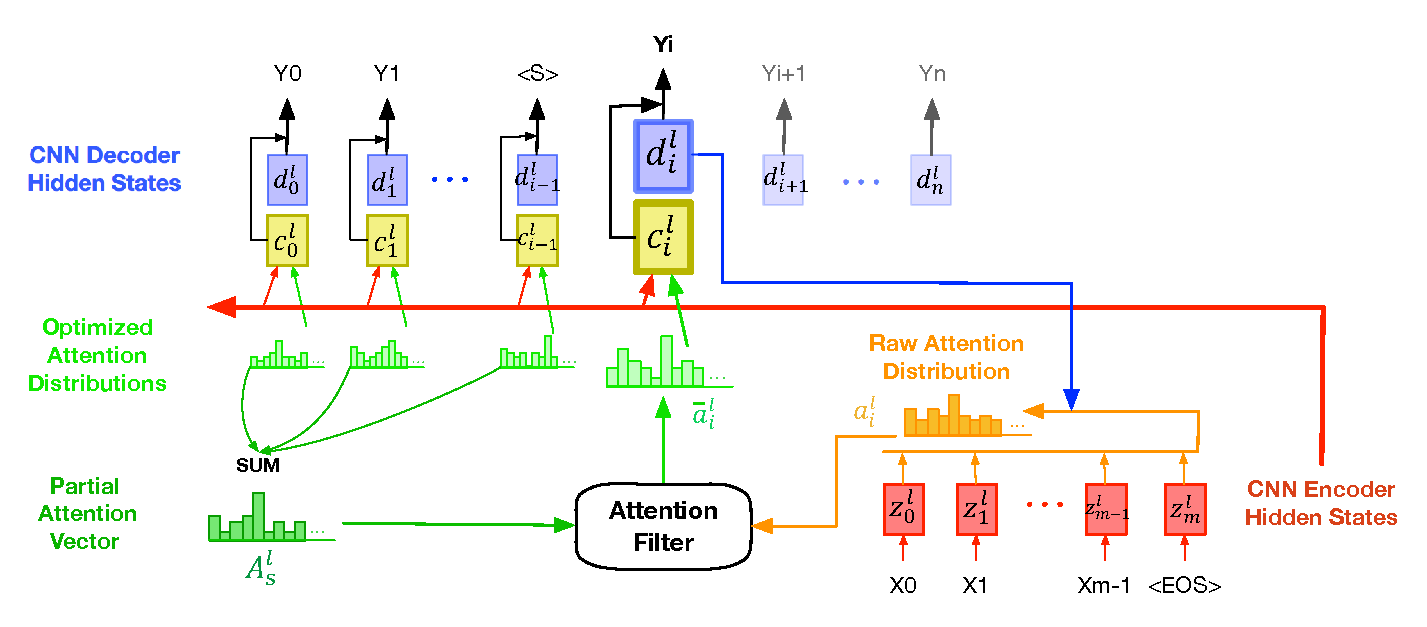
\includegraphics[width=\columnwidth]{figures/story/model}
  \caption{框架概览:我们的框架分为三个主要步骤:句子简化、句子表征和结局预测。${n_1,...n_6}$ 表示ConceptNet中的标记节点,${r_1,...r_6}$ 代表节点间的常识关系。${n_1^{'},...n_6^{'}}$ 是在ConceptNet上训练得到的对应向量。}
  \label{fig:model}
  \end{figure*}

考虑到一个包含$L$个句子 $\textbf{s} = (s_1, s_2, ..., s_L)$ 的故事情境,
我们的任务是从两个候选结局句子 $e_1$ 和 $e_2$ 中预测出正确的结局。
我们提出的方法旨在通过引入ConceptNet中的常识知识,来改进和扩展故事句子的表示,
以便更准确地预测故事结局。如\figref{fig:model}所示,该框架包括以下三个主要步骤:
句子简化(Sentence simplification)、句子表征(Sentence representation)
和故事结局预测(Ending prediction)。

\subsubsection{概念提取与句子简化}
\label{sec2:sentence_simplification}
我们的目标是从包含N个单词的输入句子 $s = {w_1, ..., w_N}$ 中提取
一系列关键概念和事件 $C_s$。我们选择ConceptNet~\cite{speer2017conceptnet} 作为这
些概念和事件的来源,因为它覆盖了广泛的常识知识。ConceptNet中的概念和事件通常由一到两
个单词的短语表达,例如``break ankle''。但在实际语境中,人们可能会使用更多样化的表达方
式,如``break her ankle''。为了弥补这种差异,我们开发了一种模糊匹配启发式方法,允许
在ConceptNet中的概念短语中加入最多 $\lambda$ 个额外单词以便在输入句子中实现模糊匹配。

面临的另一个挑战是,提取的概念可能在输入句子中相互重叠。
例如,从句子``She hope it would come back for more later''中,我们能提
取出``hope''、``\textbf{come back}''、``\textbf{come for}'' 和 ``more''等概念。在
这种情况下,我们将保留所有有意义的概念。随后,我们会从 $C_s$ 中移除那些被其他概念
完全覆盖的重复概念。例如,``come''会被``come back''覆盖,因此从列表中删除。

完整的简化算法展示在 \algoref{alg:simplify} 中,其中 $|c|$ 表示
概念 $c$ 包含的单词数量。

\begin{algorithm}[tb]
    \small
    \caption{句子简化算法}
    \label{alg:simplify}
    \textbf{Input}: ConceptNet $C$, sentence $s=\{w_1, ..., w_N\}$\\
    \textbf{Output}: Concept sequence $C_s$ 
    \begin{algorithmic}[1] %[1] enables line numbers
    \Procedure{Simplify}{$C, s$}
      \State {$C_s \gets \{\}$}
      \For {$c \in C$}
        \For {$w_i \in s$}
          \State {$t \gets \{w_i, w_{i+1}, ..., w_{i+|c|+\lambda}\}$}
          \If {$c ~\textrm{is a subsequence of}~t $}
            \State {$C_s \gets C_s + \{c\}$}
          \EndIf
        \EndFor
      \EndFor
      \For {$c_k \in C_s$}
       \If{$\exists c \in C_s \textbf{and}~\textrm{$c_k$ is contained by $c$}$}
       \State {$C_s \gets~\textrm{remove $c_k$ from}~C_s$}
       \EndIf
      \EndFor 
      \State \textbf{return} {$C_s$ }
      \EndProcedure
    \end{algorithmic}
    \end{algorithm}
    
    \subsubsection{句子表征构建}
    \label{sec2:represent}

    经过简化后,原始句子 $s$ 被转换为在 $s$ 中相同顺序的概念序列 $C_s$。这些
    概念通常通过ConceptNet中的关系连接边相互关联,实际上形成了ConceptNet的一个概念子
    图,代表着重要的结构化知识。接下来,我们将介绍对概念序列和概念子图的编码方法。这
    两种嵌入的组合成为原始输入句子的完整表示。

\subsubsection*{概念序列编码}
经过简化过程,句子的概念序列通过序列编码器 $E$ 转换为向量表示
。在本研究中,我们选用了DSSM\cite{huang2013learning}、SKBC\cite{roemmele2017rnn} 和 
BERT\cite{devlin2018bert}等带有预训练文本表示的文本分类模型。
详细信息将在\secref{sec2:baselines}中描述。为了减少编码器的词汇量,
概念序列 $C_s$ 被转换为扁平化的单词序列 $s'$,即 $C_s$ 中所有概念的
单词拼接。与原始句子相比,$s'$ 是一个简化的单词序列,已经丢弃了与常识无
关的信息。例如,在上述情况下,简化序列为``hope come back come for more''。我
们认为每个概念中的连续信息至关重要,尽管它们不构成一个连贯的句子,但仍然被保留。

然后,简化序列 $s'$ 被输入到序列编码器中,将 $s'$ 映射成一系列上下文嵌入 $H^{seq}$:
\begin{equation}
H^{seq} = E\left(s^{'}\right)
\end{equation}

\subsubsection*{概念图编码}
除了简化句子中的扁平化概念序列外,概念之间的关系对于预测
故事结局也极为重要。以往的研究\cite{chen2018incorporating,guan2018story} 已经表
明,引入ConceptNet中的结构化知识能够补充故事中的常识性推理。与现有研究不同的
是,我们不是生成手工特征,而是将结构化的常识知识直接纳入句子表征中。
Numberbatch\footnote{https://github.com/commonsense/conceptnet-numberbatch}
是ConceptNet知识图谱的预训练概念嵌入,涵盖超过2,000,000个常见概念,并在其他常
识表示任务中已被证明有效\cite{speer2017conceptnet2}。给定从句子中提取的概
念序列 $C_s$,我们将结构化知识表示 $H^{kg}$ 定义为所有概念的向量总和:
\begin{equation}
H^{kg} = \sum_{c \in C_s}{Numberbatch(c)},
\end{equation}
其中 $Numberbatch(c)$ 表示概念 $c$ 的向量。如果概念不在
Numberbatch中,我们通过平均Numberbatch中所有构成词的向量来近似其概念向量。

最终,句子 $s$ 的完整表示定义为两个组成部分的结合:$H_s=[H_s^{seq}; H_s^{kg}]$。

\subsubsection{结局预测模型设计}
\label{sec2:classifier}
为了从两个候选项中预测正确的结局,我们分别将两个候选结局与上下文句子结合起来。
我们应用不同的分类器来判断
哪个由5句话组成的故事 $\textbf{s}=(s_1, s_2, s_3, s_4, e),e\in{e_1,e_2}$ 更可能
是正确的: 
\begin{equation}
    P\left( y|s \right) = \left\{
        \begin{matrix}
        \cos \left( H_{s_{[1:4]}}, e \right) & \text{e.g., DSSM} \\ 
        \text{softmax}\left( H_{s_{[1:4]}}, e \right) & \text{e.g., BERT} \\
        \text{softmax}\left( \text{GRU}\left( H_{s_{[1:4]}}, e \right) \right) & \text{e.g., SKBC}
        \end{matrix}
    \right.
    \end{equation}
        
    其中 $H_{s_{[1:4]}}$ 是 ${s_1, s_2, s_3, s_4}$ 的表示向量。
    分类目标 $y\in{1,2}$ 对应于两个候选结局 e1 和 e2。

    通过这种方法,我们能够有效地结合常识性知识和深度学习技术,
    以更准确地预测故事的结局。通过这一框架,我们不仅提高了结局预测的准确性,
    同时也增加了对故事情境的理解深度,使得预测过程更加符合人类的常识推理方式。

%其中 $H_{s_{[1:4]}}$ 是 ${s_1, s_2, s_3, s_4}$ 的表示。分类目标 $y\in\{1,2\}$ 对应于 e1 和 e2。

\subsection{实验}
\label{sec2:experiment}

在本节中,我们将展示我们的实验设计及结果分析,以评估我们提出的方法在故事结
局预测中的有效性。首先,我们介绍了与我们方法相比较的几种基线模型,这些模型涵盖
了当前故事理解领域的多种典型技术。随后,我们深入讨论了训练和测试数据集的构建,特
别强调了新数据集的创建及其在实验中的重要作用。

实验结果和分析部分主要集中于展示不同模型在测试数据集上的表现,以及我们的简化后的概念序列编码和概
念图编码方法对提高模型性能的影响。此外,我们还比较了不同的句子简化策略,并探讨了
概念嵌入对故事结局预测的作用。最后,实验还包括了对训练数据规模和训练时间影响的分析。

总体而言,这一节旨在通过详尽的实验和细致的分析,全面展示我们方法在提高
故事结局预测准确性方面的有效性和潜力。

\subsubsection{基线模型与方法}
\label{sec2:baselines}
我们的方法与两组基线模型进行了比较。首先,正如\secref{sec2:intro}所述,
预训练的故事表征对于选择正确的故事结局非常重要。我们在三种典型的模型上应用了
基于概念的故事表征技术:DSSM、SKBC和BERT。这些模型通过不同的机制和分类方法进行预训练,
并代表了当前流行的预训练模型。


\textbf{DSSM}\cite{mostafazadeh2016corpus} 计算字符串对在连续语义空间中的相似性。
在故事结局预测任务中,DSSM将四句话的上下文和第五句话映射为语义向量,不考虑字符顺序的原始计数。
使用三个300维隐藏层对上下文和备选结局进行编码。测试时,DSSM选择余弦相似性较高的备选结局。

\textbf{SKBC}~\cite{roemmele2017rnn} 基于Skip-thought\cite{kiros2015skip},
适用于多个语义分类问题。其架构基于GRU-GRU\cite{hochreiter1997long}。我们采用与
SKBC相同的设置,但在1000节点GRU隐藏层前增加了0.4的dropout。应用二元
交叉熵函数来最大化正确结局的选择概率。所有实验均使用200的批量大小和20个训练周期。

我们在BookCorpus数据集\cite{zhu2015aligning} 上使用2400维的语言
模型\cite{kiros2015skip}\footnote{\url{https://github.com/ryankiros/skip-thoughts}} 
训练概念序列表示,该数据集包含11,038本书的文本。

\textbf{BERT}\cite{devlin2018bert},
基于Transformer\cite{vaswani2017attention} 开发,这个模型的结构我们在第一章已经介绍了。
有几种可用的预训练BERT模型,它们在模型中使用的层数和参数数量上有所不
同(基本版本有12层变压器块、768隐藏大小和12个自注意头,共计110M参数;
大型版本有24层变压器块、1024隐藏大小和16个自注意头,共
计340M参数)。我们选择了基本版本,它是在BookCorpus上预训练的。

我们的方法应用于这些模型上。对于简化方法,我们根据经验
将额外间隔 $\lambda$ 固定为1,因为更大的间隔虽然有助于发
现更多概念,但可能引入噪声。例如,在``Sally went home and wondered about her parents' marriage''中,
当 $\lambda$ 等于2和3时,我们会错误地获得``go wonder''和``go about''。
此外,结构化知识表示采用来自Numberbatch的300维向量。

第二组基准方法涵盖了多种类型的模型:这包括基于特定特征构建的方法、使用生成模型的方法,
以及一些与前述DSSM、SKBC和BERT等模型在方法论上相近的先进技术。

\textbf{FES-JOINT}\cite{peng2017joint} 结合了框架、实体和情感的特征。这个无监督的联合模型通过计算给定上下文的条件概率来选择适当的结局。

\textbf{SeqMANN}\cite{li2018multi} 考虑了多个浅层特征,包括POS标签、词嵌入、字符特征、情感否定和SemLM\cite{peng2016two}特征。

\textbf{GMSA}\cite{guan2018story} 通过多源注意力生成故事结局,并引入ConceptNet邻域信息。我们比较生成结局和两个备选结局之间的相似性。

\textbf{CGAN}\cite{wang2017conditional} 使用生成对抗网络(GAN),应用GRU生成训练数据增强的错误结局。

\textbf{SIMP}\cite{srinivasan2018simple} 使用Skip-thought句嵌入,并使用多层密集网络分类器编码整个故事,以确定正确的结局。

\textbf{GPT}\cite{radford2018improving} 通过训练文本表示的语言模型并进行线性微调,取得了巨大的进步。GPT也像BERT一样使用Transformer单元。

\textbf{ISCK}\cite{chen2018incorporating} 将情感和上下文与结局之间的常识特征纳入\cite{radford2018improving}的文本表示中,可以获得一些改进。

\textbf{TransBERT}\cite{li2019story} 不仅利用了大规模未标记数据中的一般语言知识,还利用了三个语义相关的转移任务,包括自然语言推理、情感分类和下一步动作预测,对BERT进行预训练和初始化。

\subsubsection{训练和测试数据集}
\label{sec2:dataset}
\subsubsection*{1. 数据集的选择与挑战}
在先前的研究中,为了训练故事结局预测分类模型,研究者普遍使用
了ROC验证分割,这个数据集包含3742个带有正确和错误
结局标注的项目。这些项目被进一步分割为两部分,每部分含有1871个案例,
分别作为训练集和测试集。这种方法在训练集上进行模型训练后,在测试集上取得
了良好的表现。然而,这种方法存在明显的局限性:首先,用于训练的案例数量相对较少,
可能限制了模型的学习能力;其次,由于训练集和测试集之间的偏见一致性,可能导致评估
结果不够公平或准确。

此外,\cite{sharma2018tackling}的研究指出,这些由错误结局标注
的验证集由于存在人为创作偏见,不应作为训练资源。类似地,\cite{niven2019probing}的研究发
现,BERT在论证推理理解任务\cite{habernal2018argument}中的表现完全依赖于数据集中的虚假
统计线索。这些发现表明,仅使用ROC验证分割进行训练和测试可能无法准确反映模型在实际应用中的效果。

\subsubsection*{2. 新数据集的构建}
基于以上考虑,我们决定采用不同的方法来构建训练和测试数据集。
我们的目标是创建一个新的、规模更大且更公正的数据集,以更准确地
评估故事结局预测模型的性能。这一决定得到了我们在Amazon Mechanical Turk (AMT)上征集
的ROCStories及其错误结局中的初步实验的支持。如表格\tabref{tab2:hate}所示,我们发
现特定词汇(例如``hate'')在错误结局中出现的频率远高于正确结局,暗示了潜在的信息泄露问题。
\begin{table}
  \small
  \centering
  \begin{tabular}{lccc}
  \toprule
  \textbf{数据集}& 正确结局& 错误结局 &总数\\
  \midrule
  验证集 & 3  & 70 &73\\
  测试集  & 4  & 69 &73\\
  \bottomrule
  \end{tabular}
  \caption{ROC验证集(ROC(V))和测试集(ROC(T))中单词``hate''出现在正确和错误结局的频率。}
  \label{tab2:hate}
  \end{table}

针对这一问题,我们重新评估了几种表现优异的算法以及我们的方法。
这些算法和方法仅在验证集(ROC(V))的结局部分进行训练。
ROC测试集的结果展示在\tabref{tab2:end}中。作为基线,
我们还包括了人类表现,即5名未经过验证集训练、仅凭常识判断的人
类标注者的平均准确率。人类得分远低于部分``优秀''算法的情况表明,这
些算法并非真正运用``常识'',而是依赖于训练数据中的模式。

最近发
布的修订版本$ROC_v1.5$~\cite{sharma2018tackling}
\footnote{$ROC_v1.5$ 发布在\url{https://competitions.codalab.org/competitions/15333\#participate-submit\_results},但目前已关闭,我们无法获取含有正确标签的完整数据集。我们呈现的结果是在测试阶段结束之前获取的。}
%\footnote{$ROC_v1.5$ 发布在 \url{https://competitions.codalab.org/competitions/15333#participate-submit_results},
%但目前已关闭,我们无法获取含有正确标签的完整数据集。我们呈现的结果是在测试阶段结束之前获取的。}
旨在减少ROC中的人为偏见。然而,即使在$ROC_v1.5$中,仅以结局为依据的结果仍然高
于人类表现\cite{sharma2018tackling}。此外,它只包含了规模更小的验
证集和测试集。因此,这个数据集并不一定解决了在故事闭环测试中提供合适的训练
和测试资源的问题。尽管如此,我们还是在$ROC_v1.5$上展示了我们模型的结果
(详见\secref{sec2:result})。

\begin{table}
  \small
  \centering
  \begin{tabular}{lcc}
  \toprule
  \textbf{模型}& ROC(V) (\%) &ROCS*(Tr) (\%)\\
  \midrule
  SIMP& 72.60 &59.86\\
  SKBC&72.76&58.18\\
  GPT& 77.77 &57.93\\
  $\text{TransBERT}_{\text{BASE}}$&79.0&54.52\\
  $\text{TransBERT}_{\text{LARGE}}$&75.84&54.30\\
  \midrule
  人类& 62.40&62.40\\
  \bottomrule
  \end{tabular}
  \caption{在ROC(V)和ROCS*(Tr)上仅使用结局训练的各种模型的测试准确率。}
  \label{tab2:end}
  \end{table}

%ROCStories数据集的创新使用
%为了解决这些问题,我们选择为ROCStories语料库自动添加错误结局,
%创建新的训练数据集。我们遵循了Roemmele等人\cite{roemmele2017rnn}的方法,
%通过随机和向后方法为ROC训练集中的98161个故事生成错误示例。这种方法简单但有效,
%能够生成无偏见的错误选项。我们将新生成的数据集命名为ROCS*。为了确保数据平衡,
%我们将ROCS分为训练集(ROCS(Tr))和验证集(ROCS(V)),比例为4:1。我们在
%表格\tabref{tab:end}中展示了仅使用这些结局进行机器学习的模型性能,与人类表现
%进行了比较,证明了我们重构的训练数据集的有效性。

为了解决这些问题,我们选择自动为ROCStories语料库添加错误结局,创建一个新的训练数据集。
我们遵循了Roemmele等人\cite{roemmele2017rnn}的方法,通过随机和向后方法为ROC训练集
中的98161个故事生成错误示例。随机方法将每个故事的结局替换为训练集中另一个故事的随机选定结局
,而向后方法则通过替换故事的最后一句话来生成错误示例。从这六个备选结局中(4个来自随机,
2个来自向后),我们随机选择一个以确保正确和错误数据的平衡。这样生成的数据集被称为ROCS*。
我们将ROCS分为训练集(ROCS(Tr))和验证集(ROCS*(V)),比例为4:1。

在表格\tabref{tab2:end}中,我们发现仅使用结局进行机器学习的模型表现比
人类在我们重构的训练数据集上的表现更差,这反映出了我们数据集构建的有效性。
这个数据集在一定程度上弥补了偏见信息泄露的问题。值得注意的是,在以下所有提
及的训练数据集、验证数据集和测试数据集中,我们指的是我们新创建的数
据集:ROCS*(Tr)、ROCS*(V)和ROC(T)。

\subsubsection*{3. ConceptNet的应用}
在构建新数据集的过程中,我们面临概念上的词汇表外(OOV)问题。
我们选择ConceptNet作为我们简化资源的主要原因是它覆盖了大量由多种来
源(如WordNet、DBPedia和OpenCyc)构建的常识性知识。如表格\tabref{tab:size2}所示,
在训练集和验证集中,不到0.020\%和0.017\%的结局句子完全不包含概念,这表明ConceptNet在覆盖广泛的概念领域方
面的有效性。
\begin{table}
  \small
  \centering
  \begin{tabular}{lccc}
  \toprule
  \textbf{数据集}&总故事数&上下文零概念数&结局零概念数  \\
  \midrule
  训练集& 157058 &0&26\\
  验证集&39264&0&8\\
  测试集&3742&0&0\\
  \bottomrule
  \end{tabular}
  \caption{训练集、验证集和测试集中故事(上下文和正确或错误结局)的总数和上下文或结局中不含概念的故事数。}
  \label{tab:size2}
  \end{table}

综上所述,我们通过创新地构建训练和测试数据集,并有效利用ConceptNet,
旨在提高故事结局预测模型的准确性和公正性。我们的方法强调了在减少训练数据中的偏见
和信息泄露方面的重要性,为模型的实际应用提供了更可靠的基础。
在之前的研究中,为了训练故事结局预测分类模型,

\subsubsection{实验结果和分析}
\subsubsection*{1. 端到端结果}
\label{sec2:result}

首先,我们展示了三种基线模型结合简化后的概念序列编码方法和概念图编码方法的端到端结果。
然后,我们评估了在ROC上使用新数据集训练的其他模型。

\begin{table}
\small
\centering
\setlength{\tabcolsep}{0.7mm}{
\begin{tabular}{lcccc}
\toprule
$\textbf{模型}$ &原始 (\%)&简化(\%)&概念图编码(\%)&简化+概念图编码 (\%) \\
\midrule
DSSM& 54.04&58.79&54.0&58.2 \\
SKBC&64.70&68.13&65.12&\bf{69.7} \\
$\text{BERT}_{\text{BASE(Ours)}}$&56.54&57.34& 59.43&60.24 \\
\bottomrule
\end{tabular}}
\caption{在ROC测试集上应用简化后的概念序列编码和概念图编码方法的端到端准确率。
原始=基线模型,简化=简化后的概念序列编码方法,概念图编码=概念图编码方法。}
\label{tab2:main}
\end{table}

\begin{table}
\small
\centering
\setlength{\tabcolsep}{0.7mm}{
\begin{tabular}{lcccc}
\toprule
$\textbf{模型}$ &原始 (\%)&简化(\%)&概念图编码(\%)&简化+概念图编码 (\%)\\
\midrule
DSSM& 54.30& 57.83&54.35 &58.53\\
SKBC&64.56& 67.30&65.45 &\bf{67.97}\\
$\text{BERT}_{\text{BASE(Ours)}}$&56.88&58.02&59.79&60.97\\
\bottomrule
\end{tabular}}
\caption{在$ROC_v1.5$测试集上应用简化后的概念序列编码和概念图编码方法的端到端准确率。}
\label{tab2:main1.5}
\end{table}

\tabref{tab2:main}和\tabref{tab2:main1.5}显示了所有三种典型的
预训练故事表征模型均从我们的简化后的概念序列编码方法和概念图编码方法中受益。在\tabref{tab2:main}中,
SKBC和DSSM分别通过简化后的概念序列编码方法实现了3.43\%和4.75\%的显著提升。
$\text{BERT}_{\text{BASE}}$通过简化后的概念序列编码方法获得了0.8\%的提升,通
过概念图编码方法获得了2.89\%的提升(与原始模型相比)。
这是因为BERT包含了Transformer单元,它是一种注意力机制。
BERT可以从预训练中学习信息量大的权重。
我们的简化后的概念序列编码方法甚至可以帮助减少BERT对信息量小的词的权重。
DSSM+CE(CE 是概念图编码)的表现不如DSSM,主要是因为DSSM是一个词袋模型,
它将前四个句子作为一个整体进行建模。使用概念图编码时,
我们必须将所有四个句子的嵌入求和,
然后与DSSM的输出向量连接作为最终的表征。
这样做不可避免地会丢失顺序信息。从\tabref{tab2:main1.5}
中我们也可以得出相同的结论:简化和概念嵌入可以促进故事结局的预测。

\begin{table}
\small
\centering
\begin{tabular}{lc}
\toprule
$\textbf{模型}$ & 准确率 (\%)\\
\midrule
DSSM(实现)& 54.04\\
GMSA& 61.20\\
CGAN& 60.90 \\
SeqMANN(实现)& 59.74\\
SIMP(实现)&61.09\\
FES-LM(实现)&61.60\\
ISCK(实现)& 62.21 \\
GPT(实现)& 63.46\\
SKBC(实现)&64.70\\
$\text{BERT}_{\text{BASE(Ours)}}$(实现)&56.54\\
$\text{BERT}_{\text{BASE}}$(实现)&61.46\\
$\text{BERT}_{\text{LARGE}}$(实现)&64.67\\
$\text{TransBERT}_{\text{BASE}}$(实现)&61.46\\
$\text{TransBERT}_{\text{LARGE}}$(实现)&61.89\\
\midrule
SKBC+Simp+CE(Ours)&\bf{69.7}\\
\midrule
人类& 100\\
\bottomrule
\end{tabular}
\caption{在ROC上的故事结局预测实验结果,Simp是简化后的概念序列编码,CE是概念图编码。}
\label{tab2:all-models}
\end{table}

\tabref{tab2:all-models}展示了我们新训练和验证数据集上其
他先前研究的结果(详见\secref{sec2:dataset})。
大多数基线模型都是严格按照原论文中的设置,并使用我们提出的新训练数据实现的。
$\text{BERT}_{\text{BASE(Ours)}}$使用BookCorpus重新训
练了$\text{BERT}_{\text{BASE}}$的语言模型。我们实现
的$\text{BERT}_{\text{BASE}}$和$\text{BERT}_{\text{LARGE}}$使用
我们的训练数据进行微调,并且尊重原始语言模型的参数设置。在之前的研究中SKBC有
最好的报告结果,准确率为64.7\%。
$\text{BERT}_{\text{LARGE}}$达到了64.67\%的准确率,
在所有基线中排名第二。这表明BERT在处理大量
文本数据时具有强大的学习表示能力。
我们的$\text{BERT}_{\text{BASE}}$表现不如基础
版本,因为我们仅使用BookCorpus重新
训练了语言模型。尽管更大的语料库,如维基百科,可
能带来更好的结果,但我们只是想展示
我们的简化后的概念序列编码和概念图编码方法的有效性。BERT
的不佳表现可能是由于训练数据中较少的偏
差线索所致。这与\cite{niven2019probing}的工作一致,
该工作对抗性地生成测试
集,并导致结果急剧下降。采用我们方法的SKBC达到了69.7\%的准确率,
在我们的实验中表现最佳。它比我们测试的任何其他常用模型都表现更好。
请注意,我们的实验不是为了证明某种特定算法的优越性,
而是为了展示我们提出的故事表征方法(即简化后的概念序列编码和概念图编码)
适用于多种模型。人类的表现为100\%,
可以视为上限\cite{mostafazadeh2016corpus}。所有结果都是基于5次独立运行的平均值。

\subsubsection*{2. 不同简化策略的比较}
\label{sec2:simplify}

\begin{table}
\small
\centering
\begin{tabular}{lcc}
\toprule
\textbf{事件类型} & 未应用概念图编码的准确率 (\%) & 应用概念图编码的准确率 (\%)\\
\midrule
全词(SKBC)& 64.70 & 65.12\\
\midrule
5-TUPLE&55.12 &57.83\\
FES&60.12 &63.66\\
Ours(Simp)& 68.13 &{\bf 69.70} \\
\bottomrule
\end{tabular}
\caption{在ROC上对SKBC应用不同类型事件简化后的概念序列编码的效果(未应用概念图编码)。}
\label{tab2:sse}
\end{table}

\begin{table}
\small
\centering
\setlength{\tabcolsep}{0.7mm}{
\begin{tabular}{lccc}
\toprule
\textbf{事件类型}& 简化前 & 事件 & 简化后 \\
\midrule
5-TUPLE&10.02&1&3.43\\
FES&10.02&1.52&8.95\\
Ours(Simp)&10.02&3.78&4.90\\
\bottomrule
\end{tabular}}
\caption{采用不同事件类型进行简化对词序列长度的影响。简化前 = 简化前平均词数,简化后 = 简化后平均词数,事件 = 提取的平均事件数。}
\label{tab2:size}
\end{table}

理解故事需要理解事件序列。为了评估简化后的概念序列编码方法在故事结局预测任务中的有效性,
我们比较了两种事件表征方式,即5-TUPLE\cite{pichotta2016learning}和
FES\cite{peng2017joint},它们分别依赖于依存解析或语义角色标注(SRL)。
5-TUPLE将事件表示为五元组 $(v, e_s, e_o, e_p, p)$\footnote{ROC故事使用Stanford CoreNLP工具进行5-TUPLE解析。},
其中 $v$ 是动词原形,不能为 $null$,$e_s$、$e_o$ 和 $e_p$ 分别代表主语、
直接宾语和介词宾语的名词参数,$p$ 是连接 $v$ 和 $e_p$ 的介词。另一种事
件表征FES则联合模型化不同语义知识方面:
框架\footnote{语义框架基于PropBank框架的语义角色标注注释。}、
实体和情感。与原论文不同,我们将这三个方面都以\textit{字符串}形式
而非\textit{向量}表示(例如,情感标签\textit{POSITIVE}而非情感的独热向量表示)。

\tabref{tab2:sse} 显示了在相同SKBC模型架构上应用这些简化后的概念序列编码
的效果。由于丢失过多信息,5-TUPLE只达到了55.12\%的准确率。如\tabref{tab2:size}所示,
简化后的平均词数仅为3.43。虽然FES带来了更多信息,但提取框架的流程容易导致错误传播。

\subsubsection*{3. 概念嵌入的影响}
\label{sec2:ce}
\tabref{tab2:sse} 同样表明,所有事件序列表征都能从结
合ConceptNet上预训练的概念图编码中受益。Simp和Simp+CE的结果显示
,概念之间的关联能引入额外知识,这是无法通过语言模型直接学习到的。

\subsubsection*{4. 训练数据规模}
\label{sec2:datasize}

\begin{figure}
\centering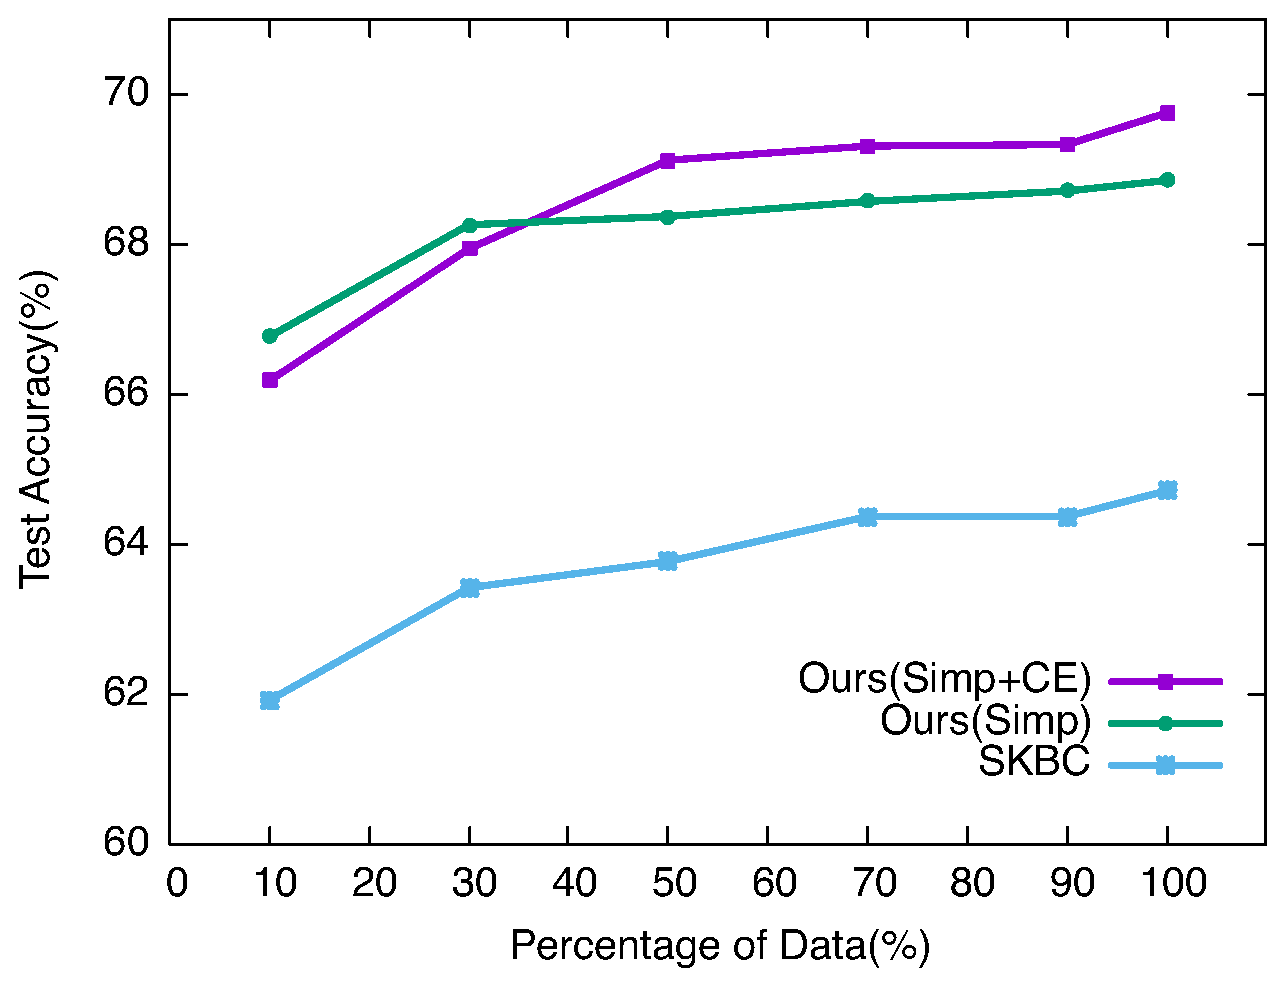
\includegraphics[width=0.8\columnwidth]{figures/story/trend}
\caption{不同训练数据规模下的准确率。}\label{fig2:trend}
\end{figure}

\figref{fig2:trend} 对比了在增加的训练数
据量(ROCS*(Tr))下,不同方法的模型性能。首先可以
看到,我们的两种方法(Simp和Simp+CE)即使在较少的训练数据下也
能表现出色。事实上,仅使用10\%的数据,它们就已经
超过了SKBC在全部数据下的准确率。其次,我们观察到与SKBC相
比,采用我们方法的模型在训练数据增加时提升更快,这一点从10\%到50\%数据量的斜率中尤为明显。
最后,比较有无概念嵌入的效果,我们发现,在没有结构化知识支持的情况下,模型难以利用更多训练数据。

\subsubsection*{5. 训练时间}
\label{sec2:time}
除了端到端准确率的提升外,简化后的概念序列编码方法还能将训练时间缩短至原来的三分
之一。这种效率提升得益于句子中词汇数量的减少和词汇表的缩小。ROC故事
中共有43,095个独特词汇,而从ConceptNet中提取的简化关键词汇仅有19,455个,这
大大减少了词汇表的大小。



\subsection{本章小结}

在本章中,我们专注于解决人工智能模型在理解和预测故事结局的任务中面临的一个核心挑战:
如何提升模型的常识性推理能力。考虑到故事理解涉及广泛而复杂的常识知识,
我们选择了故事结局预测这一特别具有挑战性的任务作为我们研究的焦点。
为此,我们提出了一种新颖的方法论,旨在通过精确识别和分析故事中的关键常识概念和事件,
从而使模型能够更深入地沿故事线索进行推理。这种方法的创新之处在于,
它不仅关注故事的表意,而且深入挖掘故事结构中的隐含逻辑和关系。

我们的方法包括三个关键部分:首先是对故事句子的简化处理,以突
出关键概念和事件;其次是基于这些关键元素构建更加丰富和细致的故事表
示;最后是运用这种表示来预测故事结局。为了实现这一目标,我们结合了句子
的概念序列编码和ConceptNet预训练的概念图编码,这一步骤对于捕捉故
事中的深层关系至关重要。

在实验部分,我们使用了一个经过精心设计的数据集,旨在减少偏见和提
高预测的准确性。我们的模型与多种现有的基线模型(如DSSM、SKBC和BERT)进
行了对比。实验结果表明,我们的方法在减少训练数据中的偏见和信息泄露方面表现
优异。此外,我们还探讨了不同的简化策略和概念嵌入的影响,
发现结合ConceptNet的预训练概念嵌入能够显著提升模型性能。

最后,本章提出了未来研究方向,主要聚焦于如何显式表示故事中的常识关系,
以提升模型对预测结果的解释能力。这种方法的发展不仅能增强模型的透明度,
还能为未来的研究提供关于故事理解和推理机制的更深刻见解。





